\documentclass{endm}
\usepackage{endmmacro}
\usepackage{graphicx}

\usepackage[utf8]{inputenc}
\usepackage[english]{babel}
\usepackage[T1]{fontenc}
\usepackage{amsmath}
\usepackage{upgreek}
\usepackage{ae}
\usepackage{color}
\usepackage{textcomp}
\usepackage{subcaption}
\usepackage{verbatim}

\usepackage{subcaption}

% The following is enclosed to allow easy detection of differences in
% ascii coding.
% Upper-case    A B C D E F G H I J K L M N O P Q R S T U V W X Y Z
% Lower-case    a b c d e f g h i j k l m n o p q r s t u v w x y z
% Digits        0 1 2 3 4 5 6 7 8 9
% Exclamation   !           Double quote "          Hash (number) #
% Dollar        $           Percent      %          Ampersand     &
% Acute accent  '           Left paren   (          Right paren   )
% Asterisk      *           Plus         +          Comma         ,
% Minus         -           Point        .          Solidus       /
% Colon         :           Semicolon    ;          Less than     <
% Equals        =           Greater than >          Question mark ?
% At            @           Left bracket [          Backslash     \
% Right bracket ]           Circumflex   ^          Underscore    _
% Grave accent  `           Left brace   {          Vertical bar  |
% Right brace   }           Tilde        ~

\newcommand{\Nat}{{\mathbb N}}
\newcommand{\Real}{{\mathbb R}}
\def\lastname{Please list your Lastname here}

\begin{document}

% DO NOT REMOVE: Creates space for Elsevier logo, ScienceDirect logo
% and ENDM logo
\begin{verbatim}\end{verbatim}\vspace{2.5cm}

\begin{frontmatter}

\title{Less is More: The Neighborhood Guided Evolution Strategies convergence on some classic neighborhood operators}

% \vspace{-1cm}

\author{Vitor N. Coelho\thanksref{address1}},
\author{Igor M. Coelho\thanksref{address2}},
\author{Nenad Mladenovi{\'c}\thanksref{address3}},
\author{Helena Ramalhinho\thanksref{address4}},
\author{Luiz S. Ochi\thanksref{address1}},
\author{Frederico G. Guimar{\~a}es\thanksref{address5}} and
\author{Marcone J. F. Souza\thanksref{address6}}

\thanks[address1]{Institute of Computation, Universidade Federal Fluminense, Niter\'oi, RJ, Brazil}
\thanks[address2]{Department of Computer Science, Universidade do Estado do Rio de Janeiro, Rio de Janeiro, Brazil}
\thanks[address3]{Mathematical Institut, SANU, Belgrade, Serbia}
\thanks[address4]{Department of Economics and Business, Universitat Pompeu Fabra, Spain}
\thanks[address5]{Department of Electrical Engineering at Universidade Federal de Minas Gerais, Brazil}
\thanks[address6]{Department of Computer Science, Universidade Federal de Ouro Preto, Ouro Preto, MG, Brazil}
\thanks[address7]{Corresponding authors: \{vncoelho, igor.machado, nenadmladenovic, helena.ramalhinho, luiz.satoru, frederico.g.guimaraes, marcone.freitas\}@gmail.com}

\vspace{-0.5cm}


\begin{abstract}
This paper extends some explanations about the convergence of a type of Evolution Strategies guided by Neighborhood Structures \cite{Coelho2016MIT}, the Neighborhood Guided Evolution Strategies.
Different well-known Neighborhood Structures commonly applied to Vehicle Routing Problems are used to highlight the evolution of the moves operators during the evolutionary process of a self-adaptive Reduced Variable Neighborhood Search procedure.
Since the proposal uses only few components for its search, we believe it can be seen inside the scope of the recently proposed ``Less Is More Approach''. 
\end{abstract}

%  in terms of response to some pre-defined load variations.
\begin{keyword}
Metaheuristics, 
Neighborhood Structure, 
Reduced VNS, 
Evolution Strategies, 
Less is More and NP-Hard problems.
\end{keyword}

\end{frontmatter}



\section{Introduction}
This paper extends the explanations regarding the Evolution Strategies applied for Combinatorial Optimization Problems, recently introduced by Coelho et al.~\cite{Coelho2016MIT}.
When introduced, the method was suggested as a novel method  that combines a search of Evolution Strategies \cite{Beyer02} in a kind of Reduced Variable Neighborhood Search (RVNS) \cite{Hansen-2008b} procedure.
In this current version, we highlight that it is a simple metaheuristic, closely related to the pioneer metaheuristic Simulated Annealing \cite{kirkpatrick1983SA}.
The similarity borders the use of random moves, however, guided by an evolutionary process instead of a cooling schedule.
The use of this basic strategies makes it to be a kind of ``Less Is More Approach'' \cite{COSTA2017247}, a simple metaheuristic framework with few parameters and mechanisms.
However, with potential of tackling several complex and large-scale combinatorial problems.

This novel study provides better explanations, acronyms, figures and more details about the proposed metaheuristic.
A classic NP-Hard problem, a real-case large-scale Vehicle Routing Problem (VRP), is used as a didactic example. 
The focus given here is to emphasize the use of important and well-know neighborhood structures: 2-opt and exchange.
These structures are often used in the resolution of the travelling salesman and vehicle routing problems.

The evolution of the evolutionary operators is discussed with details, highlighting the potential of the proposal in optimizing and adjusting its searching mechanism according to the the difficulty in improving the best known solution.
Given its main search strategy, based on Neighborhood Structures, we define the procedure as the Neighborhood Guided Evolution Strategies (NGES).

The remainder of this paper is organized as follow:
Section~\ref{sec:NGES} summarizes the main features used by the method.
Section~\ref{sec:HFVRP:HeuristicModel} describes the case of study and, in Section~\ref{subSec:HFVRP:Results}, the results for that specific problem. 
Finally, Section~\ref{sec:discussion} draws some final considerations about the possible insights presented in this study.

%%%%%%%%%%%%%%%%%%%%%%%%%%%%%

\section{The Neighborhood Guided Evolution Strategies} \label{sec:NGES}

The diagram presented in Figure \ref{fig:NGESDiagram} exemplifies the evolutionary process of the NGES.
In summary, a fixed population of size $\mu$ guides the evolutionary process, in which, random individuals from it are selected in each generation.
Each individual of the population $ind$ is composed of two additional mutation vectors, defined as $P$ and $A$, defined at Section \ref{subSec:basicPrinciples}, associated with a solution representation $s$.

The mutation phase only modifies the operators $P_i$ and $A_i$, of an individual $i$ with a previous known solution $s_i$.
After perturbing these values, i.e. self-adapting them, a systematic operation of random moves, following the rules and limits expressed in these constantly modified operators, happens.

Several offsprings are generated and a selection process happens in order to define the next population with $/mu$ individuals.

\begin{figure}[htbp]
	\center
 	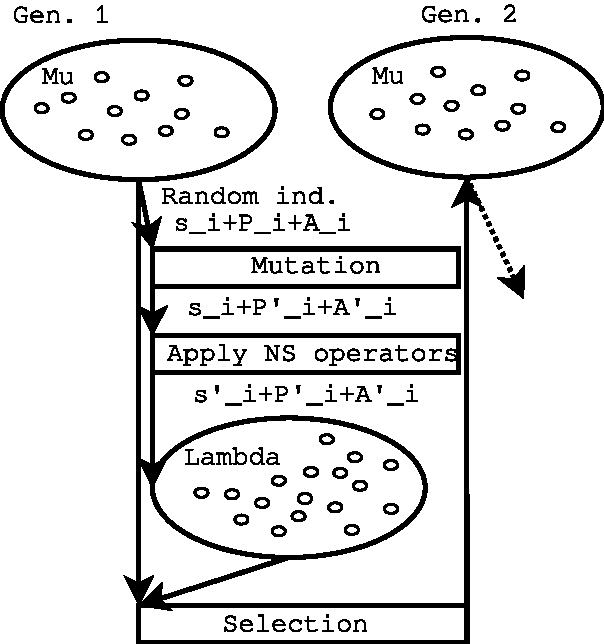
\includegraphics[width=0.6\textwidth]{./NGES_Diagram.pdf}
	\caption{NGES basic diagram} 
	\label{fig:NGESDiagram}
\end{figure}

\subsection{Basic principles \label{subSec:basicPrinciples}} 

Each individual of the population is defined as $ind  = \{ s, P, A \}$, where $P = [p_1, p_2, ..., p_i, ...,p_{neigh}]$, $A = [a_1, a_2, ..., a_j, ..., a_{neigh}]$ and $s$ is the representation of a solution for the problem.

The first mutation vector ($P_i$) defines the probability of using moves from a given NS.
In this sense, it is the likelihood associated with the application of each NS.
A given value $p^{neigh}_i \enskip \forall \enskip neigh \in |NS|$ is the current probability of applying $a^neigh_i$ moves $m \in NS_{neigh}$, in which $neigh$ is the number of available NS, and $p^{neigh}_i \in [0,1], p^{neigh}_i \in \mathbb{R}$.

As described above, the number of moves that will be applied, if a random number fits the limits $p_i$, is the corresponding value $a_i$ found inside the operator $A$.
This operator stores integer values that control the intensity of the step that will be done, once the NS is selected to be applied for modifying the solution $s_i$.
Each position $a^{neigh}_i \in [0,nap^{neigh}], a^{neigh} \in \mathbb{N}$ of this vector limits the number of applications of a given move, with $nap^{neigh}$ representing the maximum number of applications for a given move of type ${neigh} \in |NS|$.

During the mutation phase, in which each position of the vectors $P$ and $A$ are modified, classical probability distribution functions are used, such as Normal and Binomial distributions.

\section{Heterogeneous Fleet Vehicle Routing Problem with Multiple Trips} \label{sec:HFVRP:HeuristicModel}

Distribution planning is crucial for most companies that deliver goods.
Solving a VRP enable managers to find good routes to deliver their products to a set of dispersed customers.
A classical routing problem was first proposed by \cite{dantzig59}.
Here, VRP with a heterogeneous fleet of vehicles, inspired on a real case of a large distribution company, introduced by \cite{Coelho2016}, is considered.
In addition, the problem considers docking constraints, in which some vehicles are unable to serve some particular customers.
Objective functions are based on real values provided by a distribution company,
which delivers its products to 382 customers and has 169 vehicles of 8 different types.

 
\subsection{Representation and evaluation of a solution} \label{subSec:HFVRP:SolRepresentation}

A feasible solution $s$ to the HFVRPMT is represented by a set of vectors of routes, respecting each vehicle capacity and attending all costumers that need goods.
This solution is evaluated by the sum of the total fixed cost of the vehicles used plus the total cost of the customers visited and the total cost of the distances travel by the trucks.

\subsection{Neighborhood structures} \label{subSec:HFVRP:NeighStructures}

Six different neighborhood structures are applied to explore the solution space of the VRP dealt in this case study. 
The first three are intra-route movements while the last two cover inter-route. 
It is important to note that movements that lead to infeasible solutions are not allowed.
The NS are extracted from \cite{penna2013,Coelho2016}, denoted by: $NS^{2-opt}$, $NS^{Or-opt1}$, $NS^{Or-opt2}$, $NS^{Exchange}$, $NS^{Shift(1,0)}$ and $NS^{Swap(1,1)}$, briefly described bellow:

\textbf{\textit{2-opt} move.} A \textit{2-opt} move is an intra-route movement that consists in removing two non-adjacent arcs and inserting two new arcs, so that a new route is formed.
%Figure \ref{fig:EV2Opt} exemplifies the movement: edges $(4,6)$ and $(8,5)$ of Route $2$ are removed and edges $(4,8)$ and $(6,5)$ are inserted instead. 
%Note that an inversion took place involving customers $6$, $16$ and $8$, and now the sequence is 8--16--6. 
%For a symmetric problem, the total distance among these customers remains unaffected.

%%====================================================================================%
%                           Universidade Federal Fluminense                          %
%                          Mestrado em Ciência da Computação                         %
%------------------------------------------------------------------------------------%
% Título da Dissertação:                                                             %
%    Um algoritmo heurístico híbrido para o problema de roteamento de veículos com   %
%    coleta e entrega simultânea                                                     %
%------------------------------------------------------------------------------------%
% Autor      : Marcio Tadayuki Mine                           <mmine@ic.uff.br>      %
% Orientador : Luiz Satoru Ochi                               <satoru@ic.uff.br>     %
% Orientador : Marcone Jamilson Freitas Souza                 <marcone@iceb.ufop.br> %
% ADAPTADO POR: Vitor Nazario Coelho    - Maio de 2013        <vncoelho@gmail.combr> %
%====================================================================================%

\begin{figure*}[http]
	\begin{center}
		\begin{tikzpicture}[scale=.086]
			\node[depot] (n0)  at (35,35) {};
			\node[city]  (n1)  at (49,41) {};
			\node[city]  (n2)  at (17,35) {};
			\node[city]  (n3)  at (45,55) {};
			\node[city]  (n4)  at (21,53) {};
			\node[city]  (n5)  at (60,55) {};
			\node[city]  (n6)  at (60,30) {};
			\node[city]  (n7)  at (35,50) {};
			\node[city]  (n8)  at (25,22) {};
			\node[city]  (n9)  at (5,30)  {};
			\node[city]  (n10) at (40,20) {};
			\node[city]  (n11) at (65,45) {};
			\node[city]  (n12) at (10,45) {};
			\node[city]  (n13) at (5,55)  {};
			\node[city]  (n14) at (33,64) {};
			\node[city]  (n15) at (20,65) {};
			\node[city]  (n16) at (69,35) {};
			\node[city]  (n17) at (55,65) {};
			\node[city]  (n18) at (65,63) {};
			\node[city]  (n19) at (12,24) {};

			\node[depotFont]   at (n0)    {0};
			\node[cityFont]    at (n1)    {4};
			\node[cityFont]    at (n2)    {13};
			\node[cityFont]    at (n3)    {3};
			\node[cityFont]    at (n4)    {1};
			\node[cityFont]    at (n5)    {5};
			\node[cityFont]    at (n6)    {6};
			\node[cityFont]    at (n7)    {7};
			\node[cityFont]    at (n8)    {11};
			\node[cityFont]    at (n9)    {9};
			\node[cityFont]    at (n10)   {10};
			\node[cityFont]    at (n11)   {8};
			\node[cityFont]    at (n12)   {12};
			\node[cityFont]    at (n13)   {2};
			\node[cityFont]    at (n14)   {19};
			\node[cityFont]    at (n15)   {15};
			\node[cityFont]    at (n16)   {16};
			\node[cityFont]    at (n17)   {14};
			\node[cityFont]    at (n18)   {18};
			\node[cityFont]    at (n19)   {17};

			
			
			\path[->, olive] (n0)  edge (n7)
					  (n7)  edge (n14)
					  (n14) edge (n15)
					  (n15) edge (n4)
					  (n4)  edge (n13)
					  (n13) edge (n12)
					  (n12) edge (n0);

			\path[->,teal] (n0)  edge (n10)
					  (n10) edge (n8)
					  (n8)  edge (n19)
					  (n19) edge (n9)
					  (n9)  edge (n2)
					  (n2)  edge (n0);

			\path[->] 			(n0)  edge (n1);
			\path[->,dashed]	  	(n1)  edge (n6);
			\path[->] 		 	 (n6)  edge (n16)
							(n16) edge (n11);
			\path[->,dashed]		  (n11) edge (n5);
			\path[->] 		  (n5)  edge (n18)
					  (n18) edge (n17)
					  (n17) edge (n3)
					  (n3)  edge (n0);

			\node[rectangle, scale=.8, olive] at (25,47) {Route 1};
			\node[rectangle, scale=.8] at (53,47) {Route 2};
			\node[rectangle, scale=.8, teal] at (25,29) {Route 3};

			\node[depot] (m0)  at (115,35) {};
			\node[city]  (m1)  at (129,41) {};
			\node[city]  (m2)  at (97,35)  {};
			\node[city]  (m3)  at (125,55) {};
			\node[city]  (m4)  at (101,53) {};
			\node[city]  (m5)  at (140,55) {};
			\node[city]  (m6)  at (140,30) {};
			\node[city]  (m7)  at (115,50) {};
			\node[city]  (m8)  at (105,22) {};
			\node[city]  (m9)  at (85,30)  {};
			\node[city]  (m10) at (120,20) {};
			\node[city]  (m11) at (145,45) {};
			\node[city]  (m12) at (90,45)  {};
			\node[city]  (m13) at (85,55)  {};
			\node[city]  (m14) at (113,64) {};
			\node[city]  (m15) at (100,65) {};
			\node[city]  (m16) at (149,35) {};
			\node[city]  (m17) at (135,65) {};
			\node[city]  (m18) at (145,63) {};
			\node[city]  (m19) at (92,24)  {};

			\node[depotFont]   at (m0)    {0};
			\node[cityFont]    at (m1)    {4};
			\node[cityFont]    at (m2)    {13};
			\node[cityFont]    at (m3)    {3};
			\node[cityFont]    at (m4)    {1};
			\node[cityFont]    at (m5)    {5};
			\node[cityFont]    at (m6)    {6};
			\node[cityFont]    at (m7)    {7};
			\node[cityFont]    at (m8)    {11};
			\node[cityFont]    at (m9)    {9};
			\node[cityFont]    at (m10)   {10};
			\node[cityFont]    at (m11)   {8};
			\node[cityFont]    at (m12)   {12};
			\node[cityFont]    at (m13)   {2};
			\node[cityFont]    at (m14)   {19};
			\node[cityFont]    at (m15)   {15};
			\node[cityFont]    at (m16)   {16};
			\node[cityFont]    at (m17)   {14};
			\node[cityFont]    at (m18)   {18};
			\node[cityFont]    at (m19)   {17};

			\path[->, olive] (m0)  edge (m7)
					  (m7)  edge (m14)
					  (m14) edge (m15)
					  (m15) edge (m4)
					  (m4)  edge (m13)
					  (m13) edge (m12)
					  (m12) edge (m0);

			\path[->,teal] (m0)  edge (m10)
					  (m10) edge (m8)
					  (m8)  edge (m19)
					  (m19) edge (m9)
					  (m9)  edge (m2)
					  (m2)  edge (m0);

			\path[->] (m0)  edge (m1);
			\path[->,very thick]		  (m1)  edge (m11)
					  (m6)  edge (m5)
					  (m11) edge (m16)
					  (m16) edge (m6);
			\path[->]		  (m5)  edge (m18)
					  (m18) edge (m17)
					  (m17) edge (m3)
					  (m3)  edge (m0);

			\node[rectangle, scale=.8, olive] at (105,47) {Route 1};
			\node[rectangle, scale=.8] at (131,47) {Route 2};
			\node[rectangle, scale=.8, teal] at (105,29) {Route 3};

			% Legenda:
			\draw (40,15) -- (110,15);
			\draw (40,9) -- (110,9);

			\node[depot, scale=.8] at (45,12) {};
			\node[rectangle, scale=.8] at (57,12) {Depot};

			\node[city, scale=.85] at (70,12) {};
			\node[rectangle, scale=.8] at (81,12) {Client};

			\draw[->] (91,12) -- (94,12);
			\node[rectangle, scale=.8] at (102,12) {Route};

		\end{tikzpicture}
		
		\caption{Example of \textit{2-opt} Move from COELHO 2016 TODO}\label{fig:EV2Opt}
	\end{center}
\end{figure*}


\textbf{\textit{Or-optk} move.} An \textit{Or-optk} move is an intra-route movement that consists in removing $k$ consecutive customers from a given route and reinserting them into another position of the same route.
This move is a generalization of the \textit{Or-opt} proposed by \cite{or76}, in which the removal involves up to three consecutive customers only.

\textbf{\textit{Exchange} move.} An \textit{Exchange} move is an intra-route movement that consists in exchanging two customers in the same route. 

\textbf{\textit{Shift}(1,0) move.} A \textit{Shift}(1,0) move is an inter-route movement that relocates a customer from one route to another.
%Figure \ref{fig:EVShift} illustrates a \textit{Shift}(1,0) of customer $6$ originally in Route $2$ to be the first one in Route $3$.

%%====================================================================================%
%                           Universidade Federal Fluminense                          %
%                          Mestrado em Ciência da Computação                         %
%------------------------------------------------------------------------------------%
% Título da Dissertação:                                                             %
%    Um algoritmo heurístico híbrido para o problema de roteamento de veículos com   %
%    coleta e entrega simultânea                                                     %
%------------------------------------------------------------------------------------%
% Autor      : Marcio Tadayuki Mine                           <mmine@ic.uff.br>      %
% Orientador : Luiz Satoru Ochi                               <satoru@ic.uff.br>     %
% Orientador : Marcone Jamilson Freitas Souza                 <marcone@iceb.ufop.br> %
% ADAPTADO POR: Vitor Nazario Coelho    - Maio de 2013        <vncoelho@gmail.combr> %
%====================================================================================%


\begin{figure*}[http]
	\begin{center}
			\begin{tikzpicture}[scale=.086]

			\node[depot] (n0)  at (35,35) {};
			\node[city]  (n1)  at (49,41) {};
			\node[city]  (n2)  at (17,35) {};
			\node[city]  (n3)  at (45,55) {};
			\node[city]  (n4)  at (21,53) {};
			\node[city]  (n5)  at (60,55) {};
			\node[city]  (n6)  at (60,30) {};
			\node[city]  (n7)  at (35,50) {};
			\node[city]  (n8)  at (25,22) {};
			\node[city]  (n9)  at (5,30)  {};
			\node[city]  (n10) at (40,20) {};
			\node[city]  (n11) at (65,45) {};
			\node[city]  (n12) at (10,45) {};
			\node[city]  (n13) at (5,55)  {};
			\node[city]  (n14) at (33,64) {};
			\node[city]  (n15) at (20,65) {};
			\node[city]  (n16) at (69,35) {};
			\node[city]  (n17) at (55,65) {};
			\node[city]  (n18) at (65,63) {};
			\node[city]  (n19) at (12,24) {};

			\node[depotFont]   at (n0)    {0};
			\node[cityFont]    at (n1)    {4};
			\node[cityFont]    at (n2)    {13};
			\node[cityFont]    at (n3)    {3};
			\node[cityFont]    at (n4)    {1};
			\node[cityFont]    at (n5)    {5};
			\node[cityFont]    at (n6)    {6};
			\node[cityFont]    at (n7)    {7};
			\node[cityFont]    at (n8)    {11};
			\node[cityFont]    at (n9)    {9};
			\node[cityFont]    at (n10)   {10};
			\node[cityFont]    at (n11)   {8};
			\node[cityFont]    at (n12)   {12};
			\node[cityFont]    at (n13)   {2};
			\node[cityFont]    at (n14)   {19};
			\node[cityFont]    at (n15)   {15};
			\node[cityFont]    at (n16)   {16};
			\node[cityFont]    at (n17)   {14};
			\node[cityFont]    at (n18)   {18};
			\node[cityFont]    at (n19)   {17};

			\path[->, olive] (n0)  edge (n7)
					  (n7)  edge (n14)
					  (n14) edge (n15)
					  (n15) edge (n4)
					  (n4)  edge (n13)
					  (n13) edge (n12)
					  (n12) edge (n0);

			\path[->,teal, dashed] (n0)  edge (n10);
			\path[->,teal]	  (n10) edge (n8)
					  (n8)  edge (n19)
					  (n19) edge (n9)
					  (n9)  edge (n2)
					  (n2)  edge (n0);

			\path[->] (n0)  edge (n1);
	\path[->,dashed] 		  (n1)  edge (n6)
					  (n6)  edge (n16);
			\path[->] 	  (n16) edge (n11)
					  (n11) edge (n5)
					  (n5)  edge (n18)
					  (n18) edge (n17)
					  (n17) edge (n3)
					  (n3)  edge (n0);

			\node[rectangle, scale=.8, olive] at (25,47) {Route 1};
			\node[rectangle, scale=.8] at (53,47) {Route 2};
			\node[rectangle, scale=.8, teal] at (25,29) {Route 3};

			\node[depot] (m0)  at (115,35) {};
			\node[city]  (m1)  at (129,41) {};
			\node[city]  (m2)  at (97,35)  {};
			\node[city]  (m3)  at (125,55) {};
			\node[city]  (m4)  at (101,53) {};
			\node[city]  (m5)  at (140,55) {};
			\node[city]  (m6)  at (140,30) {};
			\node[city]  (m7)  at (115,50) {};
			\node[city]  (m8)  at (105,22) {};
			\node[city]  (m9)  at (85,30)  {};
			\node[city]  (m10) at (120,20) {};
			\node[city]  (m11) at (145,45) {};
			\node[city]  (m12) at (90,45)  {};
			\node[city]  (m13) at (85,55)  {};
			\node[city]  (m14) at (113,64) {};
			\node[city]  (m15) at (100,65) {};
			\node[city]  (m16) at (149,35) {};
			\node[city]  (m17) at (135,65) {};
			\node[city]  (m18) at (145,63) {};
			\node[city]  (m19) at (92,24)  {};

			\node[depotFont]   at (m0)    {0};
			\node[cityFont]    at (m1)    {4};
			\node[cityFont]    at (m2)    {13};
			\node[cityFont]    at (m3)    {3};
			\node[cityFont]    at (m4)    {1};
			\node[cityFont]    at (m5)    {5};
			\node[cityFont]    at (m6)    {6};
			\node[cityFont]    at (m7)    {7};
			\node[cityFont]    at (m8)    {11};
			\node[cityFont]    at (m9)    {9};
			\node[cityFont]    at (m10)   {10};
			\node[cityFont]    at (m11)   {8};
			\node[cityFont]    at (m12)   {12};
			\node[cityFont]    at (m13)   {2};
			\node[cityFont]    at (m14)   {19};
			\node[cityFont]    at (m15)   {15};
			\node[cityFont]    at (m16)   {16};
			\node[cityFont]    at (m17)   {14};
			\node[cityFont]    at (m18)   {18};
			\node[cityFont]    at (m19)   {17};

			\path[->, olive] (m0)  edge (m7)
					  (m7)  edge (m14)
					  (m14) edge (m15)
					  (m15) edge (m4)
					  (m4)  edge (m13)
					  (m13) edge (m12)
					  (m12) edge (m0);

			\path[->,teal, very thick] (m0)  edge (m6)
					  (m6)  edge (m10);
			\path[->,teal]	  (m10) edge (m8)
					  (m8)  edge (m19)
					  (m19) edge (m9)
					  (m9)  edge (m2)
					  (m2)  edge (m0);

			\path[->] (m0)  edge (m1);
			\path[->,very thick]  (m1)  edge (m16);
			\path[->]		  (m16) edge (m11)
					  (m11) edge (m5)
					  (m5)  edge (m18)
					  (m18) edge (m17)
					  (m17) edge (m3)
					  (m3)  edge (m0);

			\node[rectangle, scale=.8, olive] at (105,47) {Route 1};
			\node[rectangle, scale=.8] at (133,47) {Route 2};
			\node[rectangle, scale=.8, teal] at (110,29) {Route 3};

			% Legenda:
			\draw (45,15) -- (109,15);
			\draw (45,9) -- (109,9);

			\node[depot, scale=.8] at (50,12) {};
			\node[rectangle, scale=.8] at (60,12) {Depot};

			\node[city, scale=.85] at (74,12) {};
			\node[rectangle, scale=.8] at (83,12) {Client};

			\draw[->] (94,12) -- (98,12);
			\node[rectangle, scale=.8] at (104,12) {Route};

		\end{tikzpicture}
		\caption{Example of \textit{Shift}(1,0) Move}\label{fig:EVShift}
	\end{center}
\end{figure*}


\textbf{\textit{Swap}(1,1) move.} A \textit{Swap}(1,1) move is an inter-route movement that exchanges two customers from different routes.


\section{Computational experiments and analysis} \label{subSec:HFVRP:Results}

Computational experiments were carried on a Intel Core i7-3537U CPU, 2.00 GHz, with 4GB of RAM, operating system Ubuntu 14.04.

A set of five different instances was used to verify the size of the population that the NGES could perform better.
For this purpose, a batch of 30 executions was done and an ANOVA test was used to analyze the different impact of the population size ($\mu$ and $\lambda = 6\mu$).
In this ANOVA analyses, all executions were considered as blocking factors of the model, and the different objective function values between the instances were normalized and also considered in the analyses.
The null hypotheses was rejected (with $\alpha = 0.05$ and $\beta = 0.8$) and a significant difference between the population size was detected.
Figure~\ref{fig:Effects_MI_FO} shows an effect plot with 95\% of confidence level.
No significant difference was detected between the population size 50 and 100 parents.
Supporting by this conclusions, the same configuration used for the Open-Pit-Mining Operational Planning Problem, in \cite{Coelho2016MIT}, was kept:  $\mu = 100$ and $\lambda=600$.
However, the $nap_k$ limits here were relaxed and left with larger limits.

\begin{figure}[htbp]
	\center
 	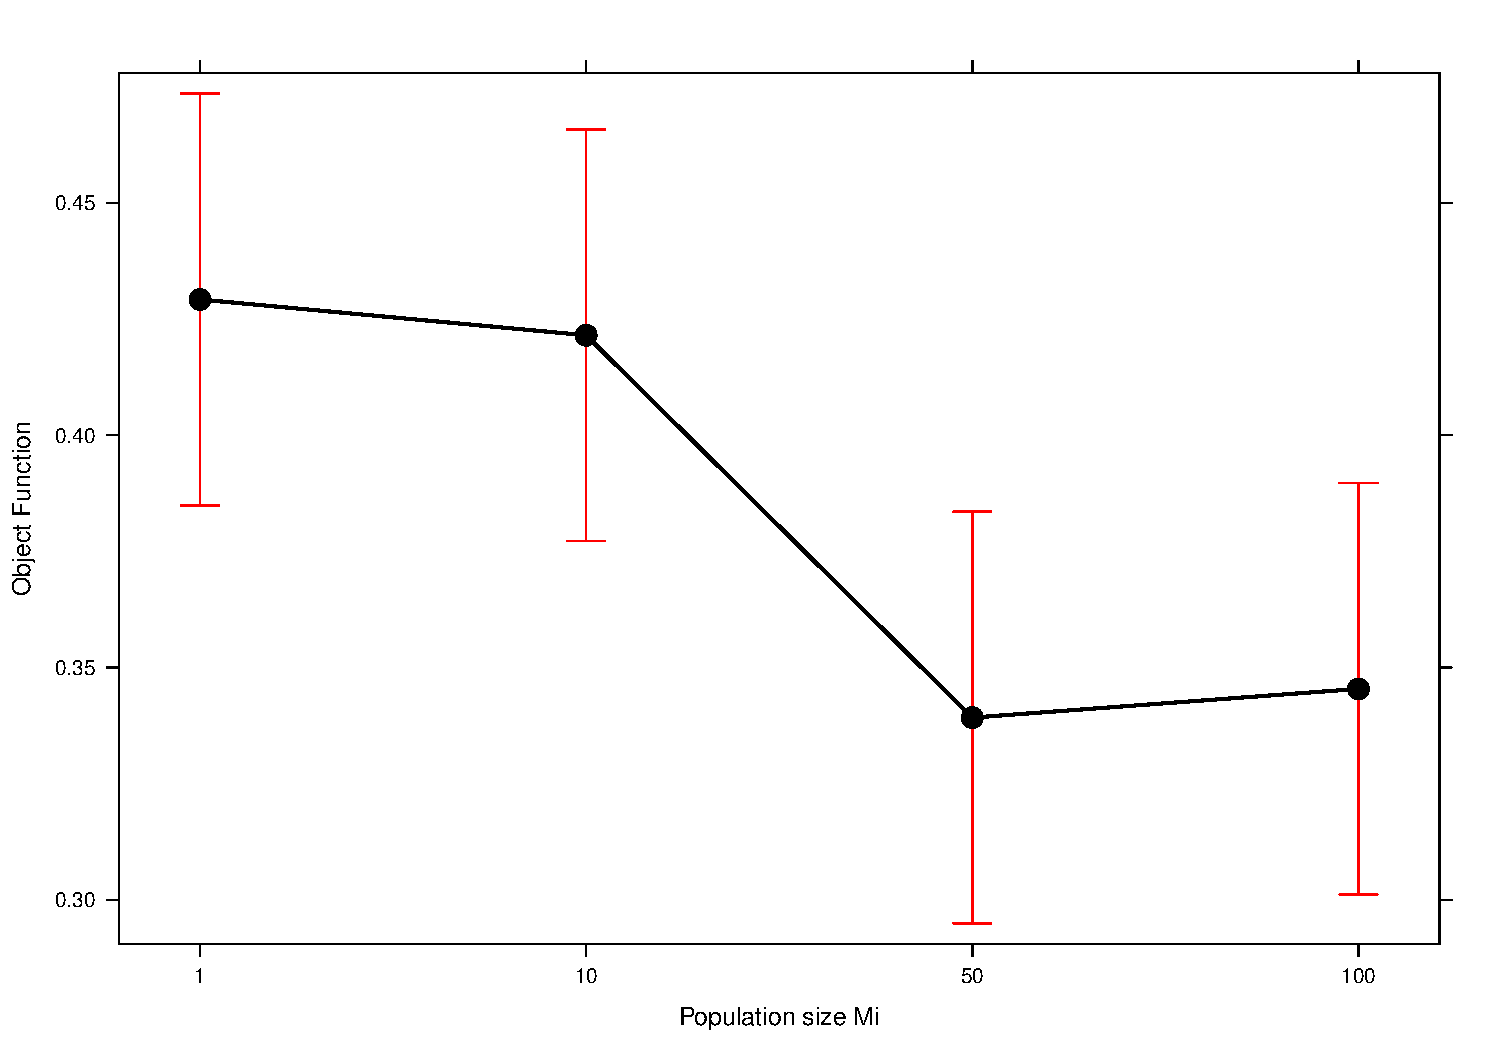
\includegraphics[width=0.6\textwidth]{./figs/HFVRP/Effects_MI_FO.pdf}
	\caption{95\% of confidence effects plot for the NGES population size on five large-scale instances of the HFVRPMT} 
	\label{fig:Effects_MI_FO}
\end{figure}

\subsubsection{Evolution strategy self-adaptive mechanism} \label{subSubSec:HFVRP:AutoAdaptiveES}

The behavior of the mutation operators for two different large scale instances is depicted in Figures \ref{fig:VRPAll}, \ref{fig:VRPSwapShiftORExchange} and \ref{fig:VRPOr2Improvements}.
It is interesting to check the ability of the NGES in increasing the number of applications of the intra-moves of neighborhoods $NS^{Shift(1,0)}$ and $NS^{Swap(1,1)}$ in order to search for new solutions, clearly seen after the first 100 generations.
For highlighting this aspect, Figure \ref{fig:VRPSwapShiftORExchange} depicts this natural ability.

\begin{figure}[t!]
%  trim={<left> <lower> <right> <upper>}
    \centering
    \begin{subfigure}[b]{0.5\textwidth}
        \centering
        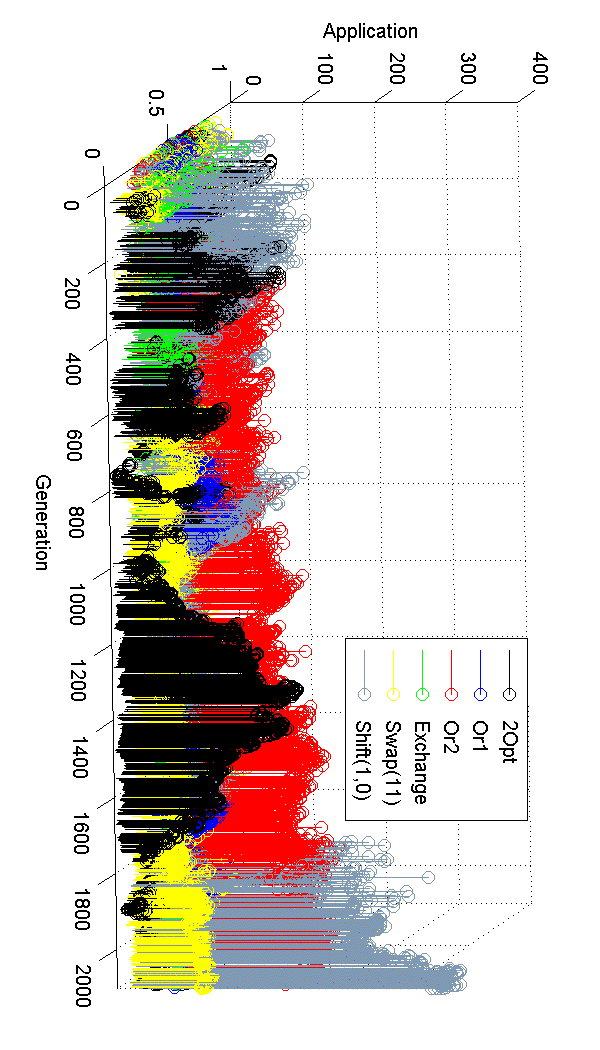
\includegraphics[angle=90,width=\textwidth]{./figs/HFVRP/VRPAll.pdf}
        \caption{Evolution of all the average values of all mutation operators \label{fig:VRPAll}}
    \end{subfigure}%
     ~
    \begin{subfigure}[b]{0.49\textwidth}
        \centering
        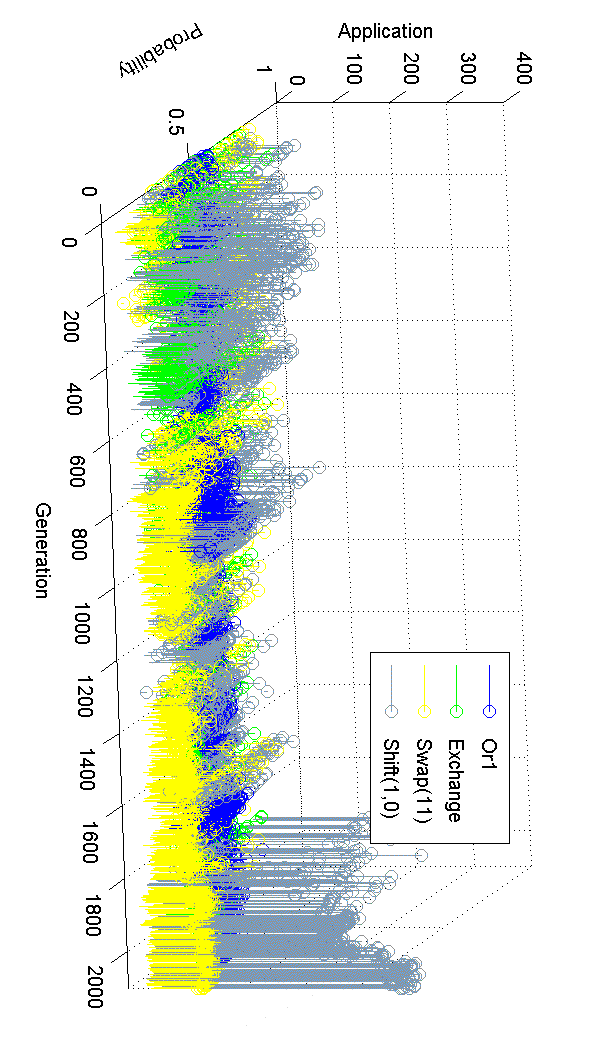
\includegraphics[angle=90,width=\textwidth]{./figs/HFVRP/VRPSwapShiftORExchange.pdf}
        \caption{Evolution of operator highlighting a specific set of NS \label{fig:VRPSwapShiftORExchange}}
    \end{subfigure}

    \caption{Stem plot showing the evolution of the mutation operators $P$ and $A$ -- Instance HFMVRPMT I}
\end{figure}


Another point that can be seen at Figure \ref{fig:VRPOr2Improvements} are the probability high peaks for $NS^{Or-opt2}$, which also coincide with the finding of new better solutions, improving the current best solution of the aforementioned execution.

\begin{figure}[htbp]
	\center
 	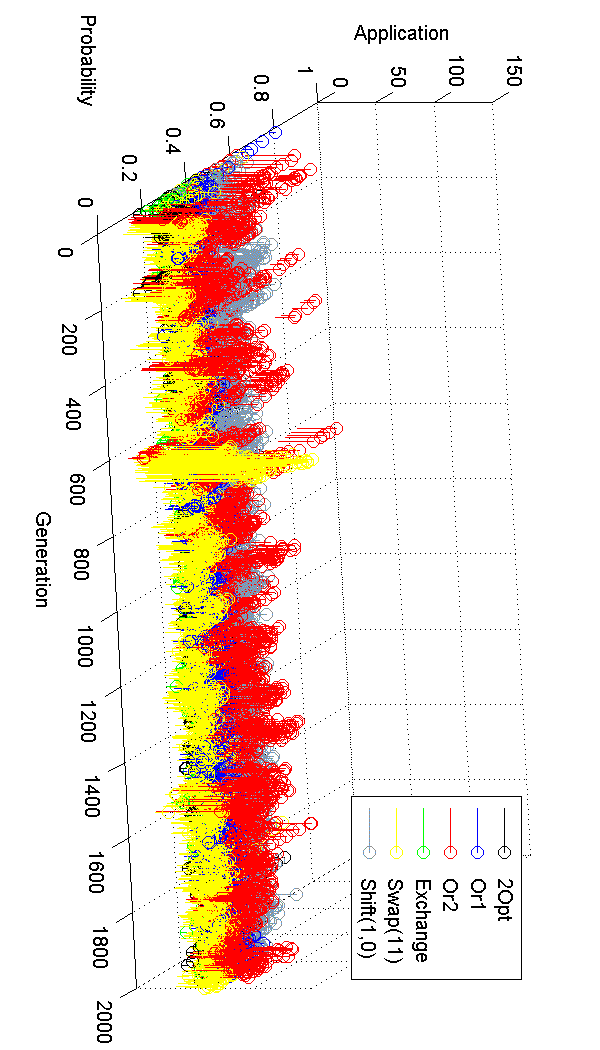
\includegraphics[angle=90,width=\textwidth]{./figs/HFVRP/VRPOr2Improvements.pdf}
	\caption{Self-adaptive operators evolution -- Instance HFMVRPMT II} 
	\label{fig:VRPOr2Improvements}
\end{figure}


%%%%%%%%%%%%
\section{Final considerations and extensions\label{sec:discussion}}

Analyzing the evolution of the range of probabilities for applying the different NS can help the comprehension of the landscape of an optimization problem.
Furthermore, the convergence showed in this study reinforces that the GES algorithm can self-regulate moves application.
As could be notice, when stucked, the operators evolve towards larger probabilities in order to perform larger changes in the solution representation.
This represents an effort for escaping from local optima.

In particular, the proposed non sophisticated strategy, basically relying on mutation operations, is an easy to implement metaheuristic but posses sufficient tools for producing successful results in real-world applications.

The method will be extended for handling Multi-objective Optimization Problems.
In this sense, it could be extension of the classic Pareto Archived Evolution Strategy \cite{knowles1999pareto}.
Basically, the only thing that should be modified is the acceptance criteria, which would storage a set of non-dominated solutions.
In this sense, the simplicity of the proposal makes its attractive for future improvements and test bed for future adjustments.
%As future extensions, this method, and also the use of neighborhood structures, could be embedded into low-cost systems, which are now in use in different activities of society daily life, in the context of our digital and interconnected smart cities.

\vspace{-0.2cm}
\section*{Acknowledgements}
Vitor N. Coelho would like to thank the support given by FAPERJ (grant E-26/202.868/2016). Marcone J. F. Souza thanks the support given by FAPEMIG and CNPq (grants CEX-PPM-00676/17 and 307915/2016-6, respectively).

\vspace{-0.2cm}
\bibliographystyle{endm}
\bibliography{otimizacao.bib}


\end{document}